\chapter{Introducci\'on}
\label{cap:introduccion}

\section{Antecedentes y motivaci\'on}
\label{intro:motivacion}

Los fenómenos que ocurren en el Universo emiten radiación electromagnética, desde las ondas de radio hasta los rayos gamma. Estas pueden ser capturadas por diversos instrumentos. Uno de estos son los interferómetros que son un conjunto de antenas que simulan ser una antena gigante \citep{AlmaInt} (Figura \Ref{fig:alma}). Un ejemplo de esto es el \textit{Atacama Large Milimeter/Submilimiter Array} (ALMA) que corresponde a un instrumento astronómico compuesto de 66 antenas de radiofrecuencia, con separaciones entre ellas que llegan hasta los 16 kilómetros \citep{AlmaWork}. 

\begin{figure}[!ht]
	\centering
	\captionsetup{justification=centering}
	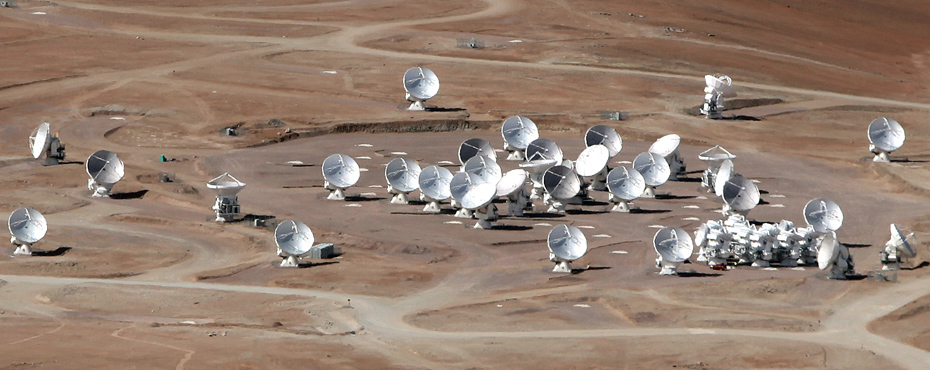
\includegraphics[scale=0.4]{images/Alma.jpg}
	\caption[Observatorio Alma.]{Observatorio Alma. Fuente: \citep{AlmaInt}}
	\label{fig:alma}
\end{figure}

Un interferómetro captura datos por cada par de antenas ($i$ y $j$) (Figura \Ref{fig:antenna}), donde el dato corresponde a la correlación compleja del campo eléctrico que se le denomina visibilidad ($V_{ij}$). Sin embargo, estas corresponden a un muestreo irregular de la transformada de Fourier del mapa de emisión del cielo (plano ($u,v$)). Es decir, esta medición no se realiza en una malla rectangular y existen grandes áreas sin valores medidos \citep{synthesis}. 

\begin{figure}[!ht]
	\centering
	\captionsetup{justification=centering}
	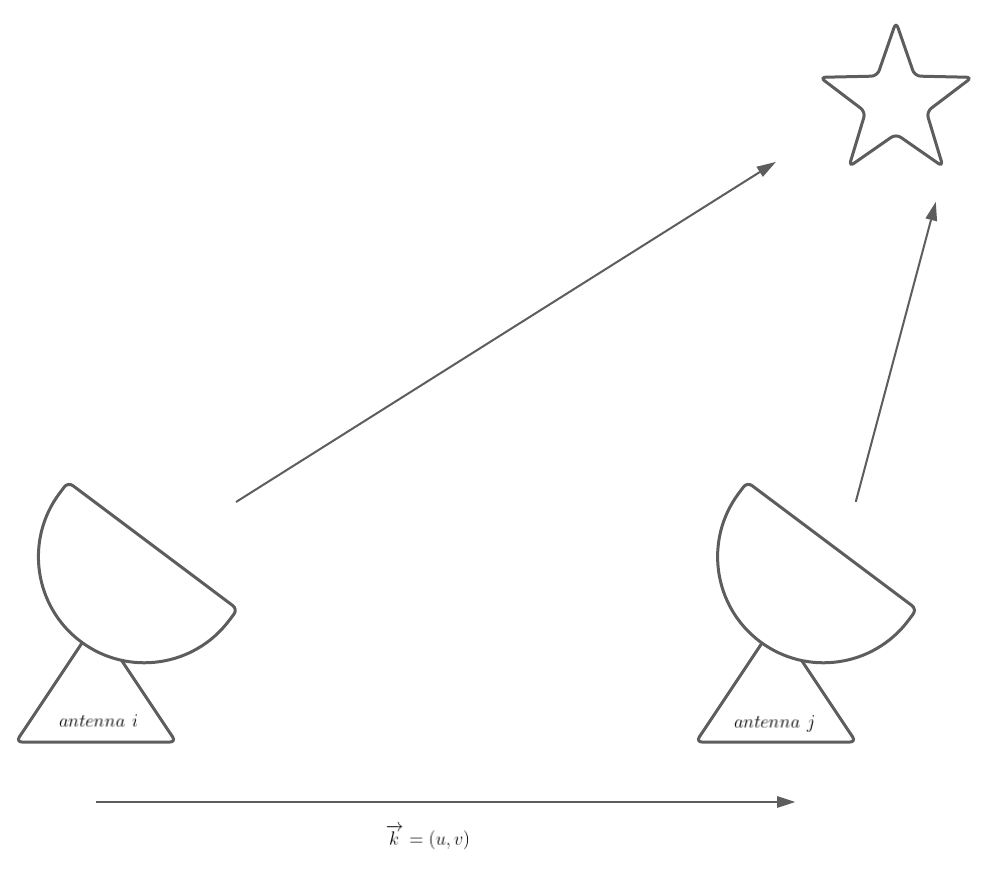
\includegraphics[scale=0.6]{images/antenna_star.png}
	\caption[Captura de datos por interferómetro.]{Captura de datos por interferómetro. Fuente: \citep{carcamo2018multi}}
	\label{fig:antenna}
\end{figure}


La base para lograr la reconstrucción de la imagen es el teorema de Van Cittert Zernike \citep{van1934wahrscheinliche}. Este describe la relación entre la visibilidad $V$ y el mapa de emisión de energía $I$ del cielo (imagen). Las coordenadas $(u,v)$ corresponden a los vectores entre las antenas medidos en metros. Esta relación indica que para obtener una imagen del cielo se debe encontrar la transformada de Fourier inversa. Sin embargo, al no tener los datos regularmente muestreados no es posible utilizar la transformada de Fourier directamente.  

\begin{equation}
    V(u, v) = \int_{-\infty}^{\infty}\int_{-\infty}^{\infty}I(x, y)e^{-2\pi i (ux + vy)}dxdy
    \label{eq:cittert-zernike}
\end{equation}

Adicionalmente, los datos que obtienen las antenas están corruptos por diferentes procesos físicos que inyectan ruido. Las turbulencias en la alta atmósfera agregan un ruido multiplicativo $(g_i)$ (ganancia) a las señales recogidas por cada antena $(i)$. Se asume que varían poco con el tiempo y son solo dependientes de la ubicación de la antena $(i)$. Los receptores de radio de cada par de antenas es afectado por un ruido termal $(\epsilon_{ij})$ Gaussiano y aditivo del instrumento, cuya desviación estándar es $(\sigma_{ij})$ y cambia por cada proceso de muestreo.

%\begin{equation}
 %   \tilde{V}_{ij}(t) = g_{i}(t)g^{*}_{j}(t)V_{ij}(t) + \epsilon_{ij}(t)
 %   \label{eq:error}
%\end{equation}

Existen muchos métodos para reconstruir una imagen a partir de las visibilidades, entre los cuales se pueden encontrar MEM  \citep{wu2012maximum} o CLEAN \citep{clean}. Dichos métodos consideran que $g_i=1$ enfocándose solamente en el ruido aditivo. Aunque existe un método llamado \textit{bispectrum} basado en el producto de tres visibilidades asociadas a tres antenas que conforman un triángulo, se demuestra que dicho producto es invariante ante perturbaciones multiplicativas de fase $(|g_i|=1)$. Esto trae consigo la ventaja de que la imagen generada es menos afectada por el ruido multiplicativo \citep{1958MNRAS.118..276J}.

El error multiplicativo puede ser reducido mediante el método de \textit{self-calibration}. Este tiene como objetivo estimar las ganancias ($g_i$) de las antenas y eliminarlas al dividir las visibilidades observadas por estas ganancias estimadas permitiendo así obtener una mejor calidad de imagen \citep{selfCalibration}. Sin embargo, requiere de un mecanismo de estimación de la imagen. La cual no se encuentra totalmente definida y el astrónomo iterativamente va seleccionando los cambios que mejoran dicha imagen de acuerdo a su conocimiento, experiencia e intuición.

Actualmente con la llegada de instrumentos que generan datos masivos como el producido por el \textit{square kilometer array} (SKA) \citep{ska}, no permitirán que la síntesis de imágenes realizada a través de programación en CPU sea óptima debido a los grandes tiempos de ejecución que se necesita \citep{carcamo2018multi, cottonGPU}. Sin embargo, una opción para incrementar los tiempos de ejecución es la computación paralela que permite realizar diversos procesos al mismo tiempo, trayendo así una ventaja sobre la programación tradicional.

\begin{comment}
Sin embargo, las tarjetas gráficas o GPU son \textit{hardware} que durante los últimos años ya no son solamente utilizadas para juegos, películas 3D e interfaces gráficas, sino que son utilizada para propósitos generales (GPGPU). Esto permite realizar tareas en GPU que tradicionalmente se realizaban en CPU, trayendo consigo la ventaja de acelerar el funcionamiento de aplicaciones de aprendizaje profundo, análisis e ingeniería. Estos dispositivos emplean una arquitectura llamada \textit{Single Instruction Multiple Thread} (SIMT) que permite ejecutar la misma instrucción en el mismo tiempo pero de manera independiente y asíncrona \citep{cheng2014professional}. 
\end{comment}

\section{Descripci\'on del problema}
\label{intro:problema}

Actualmente, la síntesis de imágenes en radio-interferometría se realiza con el framework CASA \citep{bean2022casa}. Dicho framework utiliza la heurística CLEAN tanto para generar imágenes como para calibrar los datos. El investigador en general debe realizar el proceso de calibración de manera manual. Esto tiene la desventaja de demorar el uso final de los datos para la ciencia y que la imagen generada pueda aún tener imperfecciones. Por esta razón los radio-telescopios (e.g. ALMA) disponen de un grupo de expertos con PhD en astrofísica que manualmente experimentan con los datos utilizando CASA para lograr la mejor calibración y poder entregar un producto (datos) de mejor calidad (menos ruidoso) \citep{CasaQA}. 

La nueva generación de radio-observatorios (SKA) espera producir datos a razón de 1 Tb/seg \citep{scaife2020big}. Esto hace prohibitivo el proceso manual de síntesis de imágenes. Esto incluye el proceso previo de de calibración. Es problema es mayor aún ya que dichos datos no podrán almacenarse en ningún dispositivo. Por ello que se van a reducir dichos datos utilizando una técnica llamada gridding \citep{SkaGridding}. Dicha técnica básicamente promedia los datos por celda en una malla regular. Sin embargo, el problema persiste y se requiere que el proceso de calibración sea automático.

Ante esta situación es necesario encontrar métodos y herramientas que permitan calibrar y reconstruir imágenes de buena calidad y de manera autómatica. La calidad de imagen se mide según métricas apropiadas NRMSE \citep{Chael_2018} y PSNR \citep{LiberonaTesis}. Esto enmarcándose en una herramienta que pueda generar resultados dentro de un período corto de tiempo. El método \textit{self-calibration} \citep{selfCalibration} permite eliminar el factor multiplicativo que afecta a los datos. Por otro lado las técnicas de \textit{bispectrum} permite generar algoritmos que no son afectados por el factor multiplicativo. Juntar ambos enfoques puede introducir mejoras a la solución de este problema. Es así que mediante el uso de librerías de cómputo paralelo (e.g Dask \citep{Dask_general}) y las técnicas de self-calibration con {\it bispectrum} se quiere responder a la pregunta de investigación: \textbf{¿Los resultados obtenidos de \textit{bispectrum} dentro de \textit{self-calibration} son mejores, en cuanto a calidad de imagen, que los obtenidos con otros métodos como CLEAN o MEM?}


\section{Soluci\'on propuesta}
\label{intro:solucion}

Este trabajo entrega un estudio para un posible método automático de calibración y síntesis de imágenes en radio-interferometría. Para esto se realiza la creación de módulos para los métodos de \textit{self-calibration} y \textit{bispectrum}, los cuales están dentro del framework Pyralysis \citep{winNT}, el cual está desarrollado en Python y utiliza librerías como Dask, que permite el manejo de grandes conjuntos de datos de manera perezosa, para así aplicar métodos a datos radio-interferométricos. 

Es así que se utilizarán en conjunto el método de \textit{self-calibration} y \textit{bispectrum} para reconstruir imágenes. Donde la síntesis se realiza mediante el método de máxima verosimilitud regularizada, que agrega términos regularizadores y pesos a estos, por lo que se pretende encontrar además los valores óptimos a estos. 

Cabe destacar que el método de \textit{self-calibration} se puede separar en fase y amplitud. Para este trabajo se implementará para ambos casos, donde la fase se debe encontrar los ángulos ($\theta$) que ajusten mejor la visibilidad mediante la formula de ganancias. Por otro lado, la amplitud es encontrar los mejores correcciones de ganancia a las visibilidades. Así como también existe un \textit{bispectrum} para fases y amplitudes, en este trabajo solo se enfoca en el estudio de \textit{bispectrum} en fase. 

En la teoría \citep{selfCalibration} se menciona que para obtener las ganancias asociadas en el método de \textit{Self-calibration} se debe optimizar la ecuación \ref{eq:self-calibration-intro} \citep{selfCalibration}. Sin embargo, en la actualidad las aplicaciones que ha tenido este método se realizan a través de una aproximación que es realizada mediante una divisíon de visibilidades, como es el caso de \citep{gaincal_task} y \citep{rascil}, donde una explicación de el enfoque realizado para este trabajo es detallada más adelante. 
 

%Es así que también es necesaria realizar una comparación entre estos métodos, para así comprender porque no se realiza una optimización de la ecuación \ref{eq:self-calibration-intro}.

\begin{equation}
    \sum |V_{ij} - g_{i}g_{j}^{*}\tilde{V}_{ij}|^2
    \label{eq:self-calibration-intro}
\end{equation}

Los resultados obtenidos serán comparados con los obtenidos mediante los métodos de CLEAN y MEM que son alternativas de solución a la problemática de calibración y reconstrucción de imagen que son utilizadas actualmente. Las métricas utilizadas para comparar es la raíz del error cuadrático medio (NRMSE) que evalúa las imágenes basadas en similitudes píxel a píxel y el \textit{peak signal-to-noise ratio} (PSNR) que compara el valor máximo de la señal y el valor promedio del ruido que la afecta. En la figura \Ref{fig:solucion} se puede ver una representación gráfica de la alternativa de solución propuesta.



\begin{comment}
    Los resultados obtenidos serán comparados con los métodos de CLEAN y MEM. Las métricas utilizadas para comparar es la raíz del error cuadrático medio (NRMSE) que evalúa las imágenes basadas en similitudes píxel a píxel y el \textit{peak signal-to-noise ratio} que compara el valor máximo de la señal y el valor promedio del ruido que la afecta. Así como también, esta última métrica es utilizada para detener el algoritmo de \textit{self-calibration}, ya que al tener un valor mínimo aceptable se detendrá el algoritmo logrando así una automatización del proceso. En la figura \Ref{fig:solucion} se puede ver una representación gráfica de lo propuesto.
\end{comment}

\begin{figure}[!ht]
	\centering
	\captionsetup{justification=centering}
	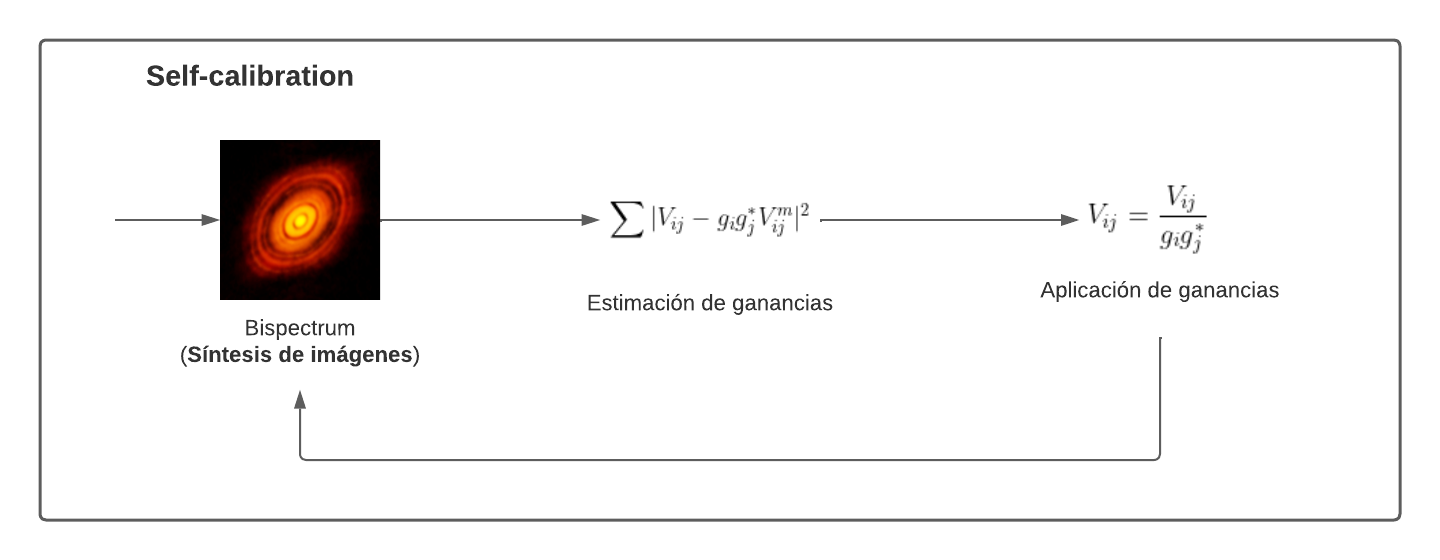
\includegraphics[scale=0.6]{images/solucion.png}
	\caption[Alternativa de solución]{Alternativa de solución. Fuente: Elaboración propia}
	\label{fig:solucion}
\end{figure}

\section{Objetivos y alcance del proyecto}
\label{intro:objetivos}

\subsection{Objetivo general}
Desarrollar una calibración de datos radio-interferometricos basada en \textit{bispectrum} para evaluar si logra una mejor calidad de imagen.

\subsection{Objetivos espec\'ificos}
\begin{enumerate}
    \item Analizar la estructura de los datos y pre-procesamiento de estos. 
	\item Automatizar la reconstrucción de imágenes en base a \textit{bispectrum} a través de un software.
    \item Incorporar el software en el framework de reconstrucción de imágenes Pyralysis.
    \item Implementar el software de reconstrucción de imágenes en base a \textit{bispectrum} usando Dask.
    \item Analizar la aplicación de \textit{Self-calibration} mediante optimización y división. 
    \item Comparar las imágenes obtenidas mediante el método de \textit{bispectrum}, con diferentes pesos de regularizadores, con aquellas reconstruidas con los algoritmos de CLEAN y MEM.
\end{enumerate}

\subsection{Alcances y limitaciones}

La solución adoptada será solamente implementada mediante el lenguaje de programación Python, utilizando el paradigma de orientación a objetos debido a que forma parte del desarrollo para el framework Pyralysis, que permite la aplicación de diversos métodos en conjuntos de datos radio-interferometricos. Además, como los conjuntos de datos a utilizar tanto para este trabajo como en el día a día son de gran tamaño, se debe utilizar la librería Dask que en si es similar a la librería de numpy, ya que contienen las mismas operaciones, pero Dask permite almacenar y trabajar con grandes conjuntos de datos. 

Por otro lado, debido al enfoque del trabajo y considerando los tiempos para este, la implementación realizada solo es se consiodera para los algoritmos de \textit{self-calibration} y \textit{bispectrum}, por lo que los algoritmos de CLEAN y MEM utilizados para comparar no son implementados, sino que se utilizan herramientas existentes como lo son \texttt{tclean} en CASA para el método CLEAN \citep{CASA_clean} y GPUVMEM para el método MEM \citep{carcamo2018multi}. 

Una limitación del software es que este solo podrá ser utilizado para datos que estén en el formato \textit{Measurement Set} (MS) \citep{kemball2000measurementset}. la cual es una base de datos para almacenar datos radio-astronómicos \citep{ms_set}.  

\section{Metodolog\'ia y herramientas utilizadas}
\label{intro:metodologia}

\subsection{Metodolog\'ia}

Para el desarrollo del trabajo toma en cuenta el método científico logrando así generar las siguientes etapas. Cabe destacar que en cada etapa se puede volver hacia alguna anterior de ser necesario. 

\begin{itemize}
    \item \textbf{Investigación}: Corresponde al estudio de los distintos parámetros que afectan los métodos de \textit{self-calibration} y \textit{bispectrum} para así ser implementados, tomando en cuenta así también el trasfondo teórico detrás de estos parámetros. 
    
    \item \textbf{Desarrollo}: En esta etapa se contempla el variar los distintos tipos de parámetros estudiados anteriormente para así obtener la composición que entregue la mejor imagen reconstruida. Para esto se utilizará el \textit{peak signal-to-noise ratio} (PSNR) para saber la calidad de estas.
    
    \item \textbf{Experimentación}: Se realiza la reconstrucción de imágenes a través de \textit{self-calibration} y \textit{bispectrum}, con los parámetros encontrados anteriormente. Además, se realiza la reconstrucción de imágenes mediante \textit{self-calibration} junto a MEM y CLEAN. 
    
    \item  \textbf{Análisis}: Se realiza el estudio y comparación entre las imágenes obtenidas con los distintos métodos mencionados en la etapa de experimentación. Para comparar se utilizará el PSNR o NRMSE de cada una de las imágenes obtenidas mediante los distintos métodos. 
\end{itemize}

Considerando las etapas anteriormente mencionadas, se decide utilizar una metodología ágil, de tal manera de realizar ciclos cortos para entregar avances durante el desarrollo del proyecto. Es así que la metodología utilizada es la denominada metodología en espiral que fue propuesta en \cite{10.1145/12944.12948}, que establece una combinación del enfoque en cascada y el enfoque iterativo. Esta metodología se caracteriza por tener una serie de ciclos de desarrollo que forman una espiral (Figura \ref{fig:spiral_method}), donde cada ciclo consta comúnmente de cuatro fases principales denominadas: Determinación de Objetivos, Análisis del riesgo, Desarrollar y probar y Planificación. De esta manera estas etapas son reemplazadas por las etapas de Investigación, desarrollo, experimentación y análisis mencionadas inicialmente, además que en estas etapas se consideran reuniones con el profesor guía y co-guía para el análisis de avances y problemáticas del desarrollo. 

\begin{figure}[!ht]
	\centering
	\captionsetup{justification=centering}
	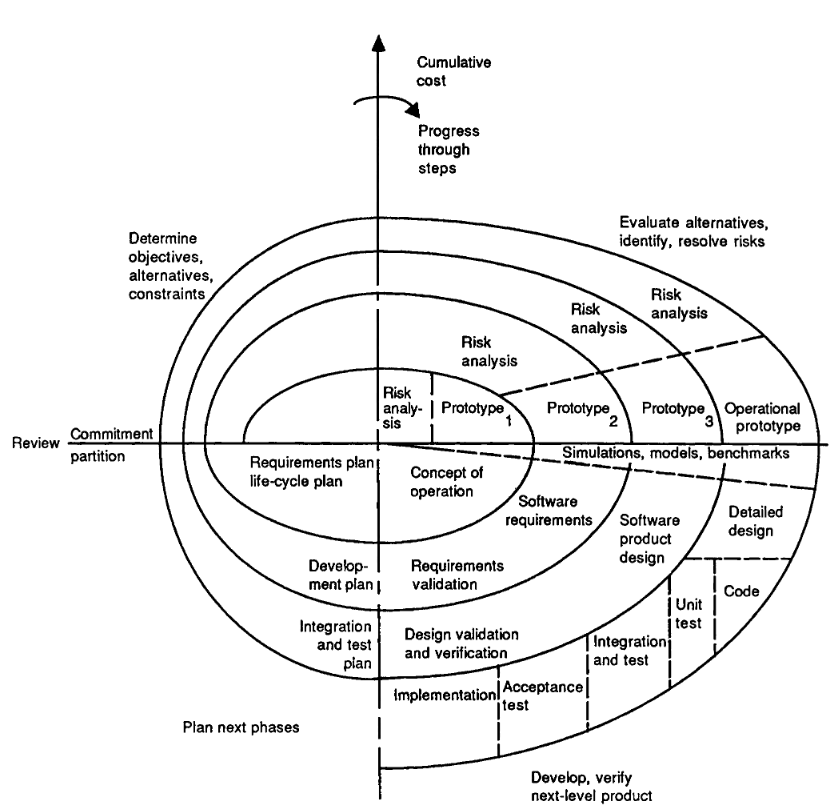
\includegraphics[scale=0.4]{images/Hoen_spiral.png}
	\caption[Metodología en espiral]{Metodología en espiral. Fuente: \citep{10.1145/12944.12948}}
	\label{fig:spiral_method}
\end{figure}

\subsection{Herramientas de desarrollo}

Para el desarrollo de la solución se utilizarán las siguientes herramientas.

\begin{itemize}
    \item \verb|Ubuntu 18.04|: Sistema operativo Linux basado en Debian. 
    \item \verb|Python|: Lenguaje de programación de alto nivel interpretado, que se utilizará junto al paradigma de orientación a objetos (POO).
    \item \verb|numpy|: Librería enfocada en la computación científica de Python.
    \item \verb|dask|: Librería que permite el computo científico de manera paralela en Python.
    \item \verb|numba|: Librería que permite la compilación \textit{Just-in-time}(JIT), que soporta operaciones \texttt{numpy} y \texttt{cupy}.
    %\item \verb|cupy|: Es una libreia de Python que permite la computación acelerada mediante GPU.
    \item \verb|CASA|: Es un software de procesamiento de datos desarrollado por ALMA, que permite el trabajar con datos de antenas radio-interferometricas. 
    \item \verb|GPUVMEM|: Es un framework que permite sintetizar imágenes utilizando una aproximación Bayesiana para resolver el problema.
    \item \texttt{TaQL}: Es un lenguaje de programación similar a SQL que permite realizar operaciones sobre tablas del tipo MS. Su siglas vienen del nombre completo \textit{Table Query Language}.
    \item \texttt{Pyralysis}: Es una librería de Python que combina el uso de este lenguaje con el poder de otras herramientas como Dask para aplicar diferentes métodos a conjuntos de datos radio-interferométricos.  
    \item \texttt{Visual studio code}: Es un editor de código que permite el uso de extensiones que ayudan al desarrollo.
\end{itemize}


Se consideran dos ambientes de trabajo. El primero corresponde al computador personal para el desarrollo del código, donde las especificaciones de este son las siguientes. 

\begin{itemize}
    \item Procesador IntelCore i5-11400.
    \item 32 GB de memoria RAM. 
    \item NVIDIA GeForce GTX 3060ti 8GB
    \item 2 HDD 1TB
    \item 1 SSD 258GB
\end{itemize}

La segunda estación de trabajo considerada es el servidor del departamento de ingeniería informática de la universidad de Santiago de Chile, utilizado para la ejecución de pruebas. Las características de este son las siguientes. 

\begin{itemize}
    \item 2 procesadores Xeon E5-2640.
    \item 256 GB de memoria RAM. 
    \item 4 tarjetas Tesla P100 con SXM2.
    \item 2 HDD 4TB
\end{itemize}


\section{Organizaci\'on del documento}
\label{intro:organizacion}

El documento se organiza de la siguiente manera. En el capítulo 2 se presentan los conceptos básicos para comprender la problemática y solución de este trabajo. Luego en el capítulo 3 se da a conocer el estado actual de implementación que han tenido los métodos de \textit{self-calibration} y \textit{bispectrum}. Siguiente a este, en el capítulo 4, se muestra el análisis necesario para la aplicación de los métodos y siguiente a este, en el capitulo 5 se muestra la implementación realizada según lo visto en el análisis. En el capitulo 6, se muestra los experimentos realizados con las imágenes y métricas asociadas, para luego ser discutidos en el capitulo 7. Finalmente, en el capitulo 8 se mencionan todas las conclusiones sobre el trabajo realizado. 